\documentclass{article}
\usepackage{graphicx,fancyhdr,amsmath,amssymb,amsthm,subfig,url,hyperref,epigraph,lipsum,wrapfig}
\usepackage[margin=1in]{geometry}
\setlength\epigraphwidth{.8\textwidth}

% Bibliography
\usepackage[backend=biber, style=authortitle-comp, maxcitenames=1, refsection=section]{biblatex}
\addbibresource{report.bib}

%----------------------- Macros and Definitions --------------------------

\renewcommand{\theenumi}{\bf \Alph{enumi}}

\fancypagestyle{plain}{}
\pagestyle{fancy}
\fancyhf{}
\fancyhead[RO]{\sffamily\large University of Delhi}
\fancyhead[LO]{\sffamily\large MCS-204 Advanced Computer Networks}
\fancyfoot[RO]{\sffamily\thepage}
\renewcommand{\headrulewidth}{1pt}
\renewcommand{\footrulewidth}{1pt}

\graphicspath{{figures/}}

%-------------------------------- Title ----------------------------------

\title{Emerging Trends in Mobile Communications}
\author{
    Samyak Ahuja \\
    \texttt{Class ID: 29}
    \and
    Mayank Kharbanda \\
    \texttt{Class ID: 16}
}

%--------------------------------- Text ----------------------------------

\begin{document}
\maketitle

%--------------------------------- Title ----------------------------------
\section{Centralized-RAN}

\epigraph{Technology offers us a unique opportunity, 
though rarely welcome, to practice patience.}
{\parencite{patience12}}

%--------------------------------- Intro ----------------------------------
\subsection{Introduction}

Global mobile data traffic is increasing at a substantial rate. 
It is estimated by \textcite{cisco19} that it will grow seven fold
from 2017 to 2022, with cell network advances and cut off in 
data price. To satisfy the consumer demands the network capacity 
is to be increased. It can be done by adding cell sites or by 
implementing the techniques like Multiple Input Multiple 
Output(MIMO). But increasing cell sites requires high capital 
investment and also results in increase in interference.
\nocite{checko14}


%------------------------------ Architecture -----------------------------
\subsection{Architecture}


%------------------------------ Traditional -------------------------------
\subsubsection{Traditional Macro Base}


In the traditional architecture(Figure 2a), radio and baseband
processing is done inside a base station. The antenna module 
is generally located near the radio module, coaxial cables
are used to connect them, signal loss associated with them is 
high. This architecture was popular during 1G and 2G mobile 
networks.\nocite{checko14}



%--------------------------------- RRH ----------------------------------
\subsubsection{Base station with RRH}


In the Remote Radio Head (RRH) architecture(Figure 2b), the base station 
has two components namely, a radio unit and a signal processing 
unit. The radio unit is called a RRH or Remote Radio Unit (RRU).
The signal processing part is called a BBU or Data Unit (DU). 
This architecture was introduced during 3G networks and right now 
the majority of base stations use it.\\


The distance between a RRH and a BBU can be extended up to 40 km,
where the limitation is coming from processing and propagation delay.
In this architecture, the BBU equipment can be placed in a more 
convenient place, enabling cost savings on site rental and 
maintenance compared to the traditional RAN architecture. 
RRHs can be placed up on poles, leveraging efficient cooling and
saving on airconditioning in BBU housing. One BBU can serve many
RRHs. RRHs can be connected to each other in a daisy chained 
architecture. Common Public Radio Interface (CPRI) is the 
radio interface protocol widely used for IQ data transmission
between RRHs and BBUs.(Figure \ref{fig:RRH_BBU_CRAN})\nocite{checko14}



\begin{figure}[!h]
  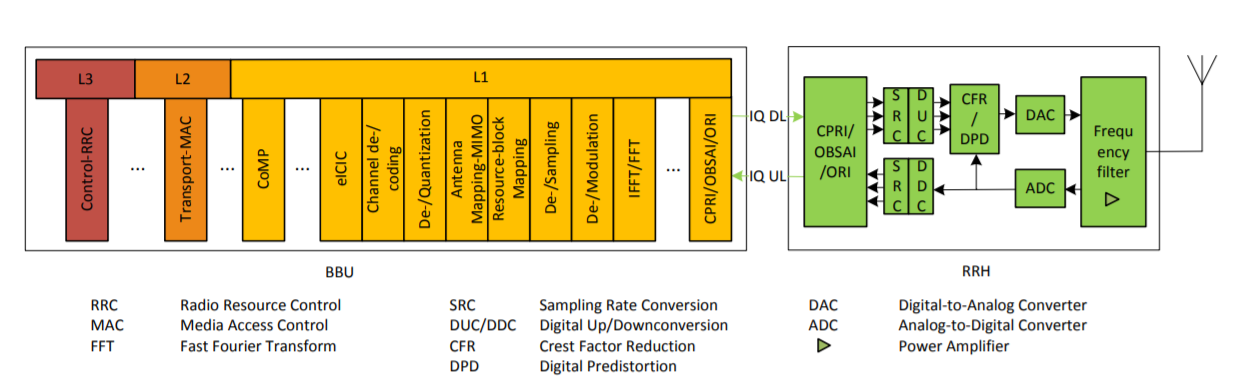
\includegraphics[width=\linewidth]{res/RRH_BBU_CRAN.PNG}
    \caption{Sub modules of BBU and RRH. Source: \parencite{checko14}}
  \label{fig:RRH_BBU_CRAN}
\end{figure}



\begin{wrapfigure}{l}{0.5\textwidth}
  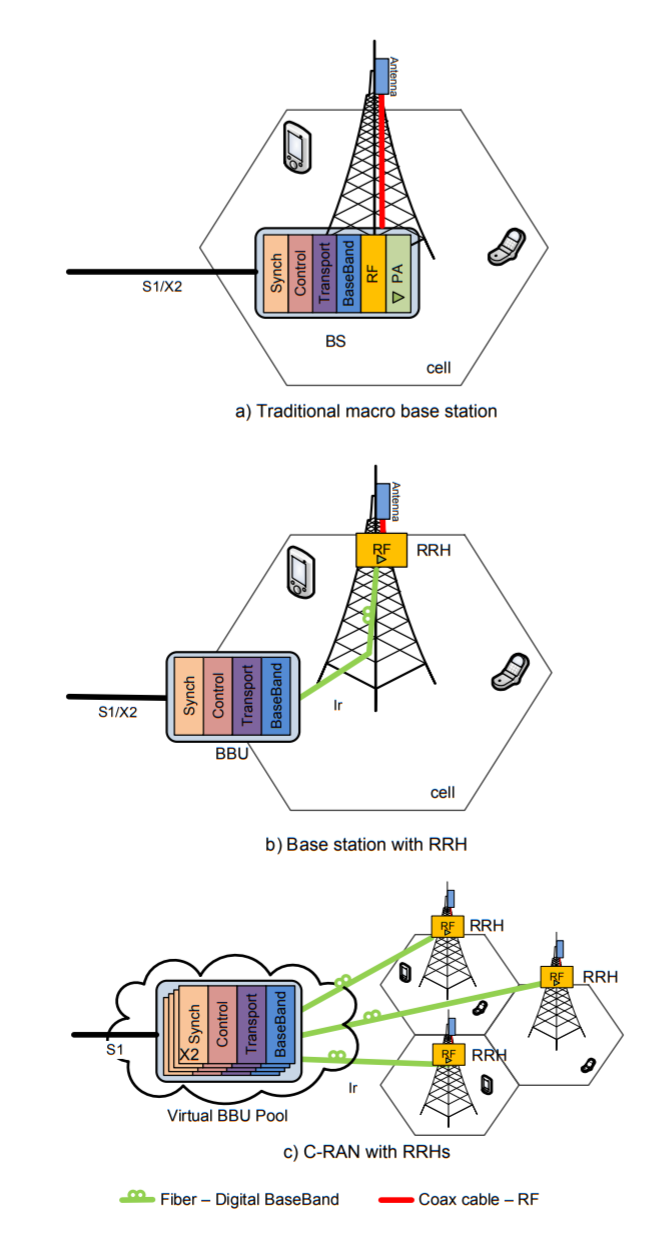
\includegraphics[scale=0.5]{res/compare_arc_CRAN.PNG}
    \caption{Base station architecture evolution.
    Source: \parencite{checko14}}
  \label{fig:compare_arc_CRAN}
\end{wrapfigure}



%--------------------------------- C-RAN ----------------------------------


\subsubsection{Centralized base station architecture, C-RAN} 

In C-RAN(Figure 2c), in order to optimize BBU utilization between
heavily and lightly loaded base stations, the BBUs are 
centralized into one entity that is called a BBU Pool.
A BBU Pool acts as a virtualized cluster to perform baseband 
processing. The concept of C-RAN was first introduced by IBM
under the name Wireless Network Cloud (WNC) and builds
on the concept of Distributed Wireless Communication System.
Since then various companies exploited the architecture and 
proposed improvements.\\


Figure \ref{fig:LTE_CRAN} shows an example of a C-RAN mobile LTE
network. The fronthaul part of the network spans from the
RRHs sites to the BBU Pool. The backhaul connects the BBU
Pool with the mobile core network. At a remote site, RRHs are
co-located with the antennas. RRHs are connected to the high
performance processors in the BBU Pool through low latency,
high bandwidth optical transport links. Digital baseband, i.e.,
IQ samples, are sent between a RRH and a BBU.\nocite{checko14}



%------------------------------ Advantages --------------------------------

\subsection{Advantages}\nocite{cmri11}

\begin{description}
    
    \item [Energy Efficient and Cost-saving] With centralized 
    processing, the number of BS sites can be reduced. Thus 
    the air conditioning and other site support equipment's 
    power consumption can be largely reduced.\\ 
    As the BBU pool is a shared resource among a large number
    of virtual BS, it means a much higher utilization rate of
    processing resources and lower power consumption can be
    achieved.
    
    \item [Capacity Improvement] In C-RAN, virtual BS's can work
    together in a large physical BBU pool and they can easily 
    share the signaling, traffic data and channel state 
    information (CSI). 
    
    \item [Adaptability to Non-uniform Traffic] C-RAN is also
    suitable for non-uniformly distributed traffic due to the 
    load-balancing capability in the distributed BBU pool.
    
\end{description}


%------------------------------ Challenges --------------------------------

\subsection{Challenges}\nocite{checko14}

\begin{description}
    
    \item [Bandwidth, Latency and Jitter] C-RAN brings a huge
    overhead on optical links between RRH and BBU pool as shown
    in figure \ref{fig:RRH_BBU_CRAN}.
    The transport network not only needs to support high bandwidth 
    and be cost efficient, but also needs to support strict latency 
    and jitter requirements.
    
    \item [BBU cooperation, interconnection and clustering] 
    There is a need to improve the performance between BBUs. 
    Cells should be optimally clustered to be assigned to one
    BBU Pool, in order to achieve statistical multiplexing gain,
    facilitate CoMP, but also to prevent the BBU Pool and the
    transport network from overloading. 
    
    \item [Virtualization technique] A virtualization technique
    needs to be proposed to distribute or group processing between
    virtual base station entities and sharing of resources among 
    multiple operators. Any processing algorithm should be 
    expected to work real time - dynamic processing capacity 
    allocation is necessary to deal with a dynamically changing
    cell load.
    
\end{description}



\begin{wrapfigure}{r}{0.5\textwidth}
  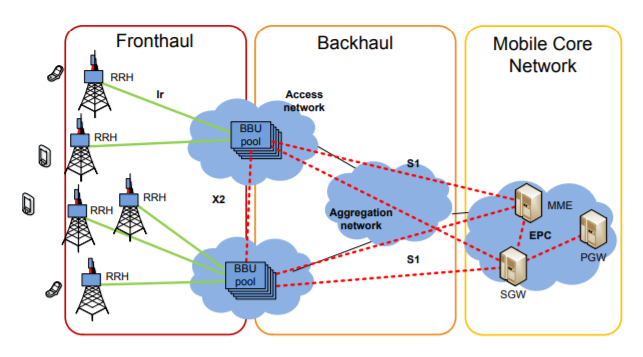
\includegraphics[scale=0.7]{res/LTE_CRAN.PNG}
    \caption{C-RAN LTE mobile network. Source: \parencite{checko14}}
  \label{fig:LTE_CRAN}
\end{wrapfigure}



%--------------------------------- Future --------------------------------


\subsection{C-RANs towards 5G}\nocite{peng16}


It is envisioned that 5G will bring a 1000x increase in terms 
of area capacity compared with 4G, achieve a peak rate in
the range of tens of Gbps, support a roundtrip latency of
about 1 ms as well as connections for a trillion of devices,
and guarantee ultra reliability.\\

The field trials conducted by China Mobile have verified the
throughput gain brought by C-RANs based on an uplink LTE model,
reaching up to near 300\%. Through dense RRHs in C-RANs,
massive connections are efficiently supported, and it is not
hard to provide good service for trillion of devices if the
density of RRHs is sufficiently high. Although a big gap
is still observed compared to 5G requirements, the result
has shown the potential advantages of C-RANs. Meanwhile,
different advanced techniques can be involved in C-RANs to
further improve the spectrum efficiency.

%--------------------------------- Bib ----------------------------------

\printbibliography[heading=subbibliography]

\end{document}
